%% PNAStwoS.tex
%% Sample file to use for PNAS articles prepared in LaTeX
%% For two column PNAS articles
%% Version1: Apr 15, 2008
%% Version2: Oct 04, 2013

%% BASIC CLASS FILE
\documentclass{pnastwo}

%% ADDITIONAL OPTIONAL STYLE FILES Font specification

%\usepackage{pnastwoF}



%% OPTIONAL MACRO DEFINITIONS
\def\s{\sigma}
%%%%%%%%%%%%
%% For PNAS Only:
\url{www.pnas.org/cgi/doi/10.1073/pnas.0709640104}
\copyrightyear{2015}
\issuedate{Issue Date}
\volume{Volume}
\issuenumber{Issue Number}
%\setcounter{page}{2687} %Set page number here if desired
%%%%%%%%%%%%

\begin{document}

\title{Subjectivity predicts adjective ordering preferences}

\author{Gregory Scontras\affil{1}{Department of Psychology, Stanford University, Stanford, CA 94305},
Judith Degen\affil{1}{},
\and
Noah D.\ Goodman\affil{1}{}}

\contributor{Submitted to Proceedings of the National Academy of Sciences
of the United States of America}

%%%Newly updated.
%%% If significance statement need, then can use the below command otherwise just delete it.
\significancetext{Speakers exhibit robust ordering preferences when it comes to modification involving more than one adjective. We present experimental and corpus results showing that these preferences track the subjectivity of the adjectives at play such that less subjective adjectives occur closer to the nouns they modify.}

\maketitle

\begin{article}
\begin{abstract}
{Abstract here\ldots}
\end{abstract}

\keywords{language | ordering preferences | subjectivity | faultless disagreement}

%\abbreviations{SAM, self-assembled monolayer; OTS, octadecyltrichlorosilane}

\dropcap{I}ntoduction\ldots summary of the literature on adjective ordering preferences.


\section{Corpus Counts}

Description of our corpus work.

\begin{figure}[h]
	\centering
	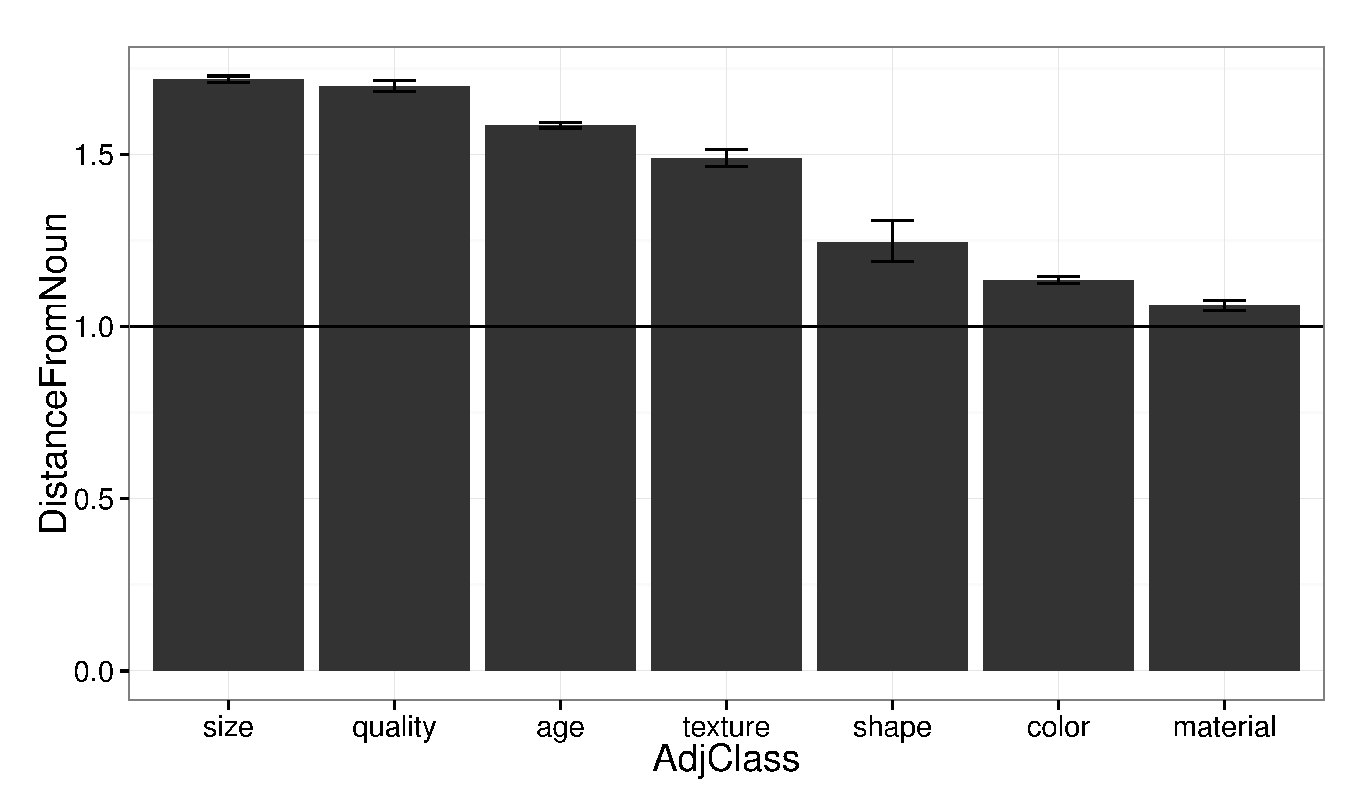
\includegraphics[width=.95\linewidth]{plots/distance_from_noun.eps}
	\caption{Average distance from noun by adjective class for cases with at least two modifying adjectives (39,199 cases).}\label{distance-from-noun}
\end{figure}

Based on the average distance-from-noun scores calculated in Fig.\ \ref{distance-from-noun}, we may infer the ordering preferences in \ref{inferred-order-preferences}.
\be size \geq quality > age > texture > shape > color > material \label{inferred-order-preferences}\ee

\section{Behavioral Experiments}
	
\subsection{Subjectivity} We conducted experiment 1 to measure the subjectivity of adjectives and the broader classes to which they belong. Participants evaluated the potential for faultless disagreement between two differing descriptions of an object (\emph{Experiment 1a: Faultless Disagreement}). For example, an experimental trial might have Mary assert ``that apple is old,'' then have Bob counter with ``that apple is not old.'' To the extent that both Mary and Bob can be right in their descriptions of the apple, ``old'' admits that degree of faultless disagreement. In other words, to the extent that two people might disagree about a description without one necessarily being wrong, that description is subjective. We validated our faultless disagreement measure in a separate paradigm, which explicitly asked about the potential ``subjectivity'' of an object description like ``old apple'' (\emph{Experiment 1b: Subjectivity}). The results of these two methods are highly correlated with each other ($r^{2} = 0.89$), suggesting that the measures they invoke converge in their estimation of adjective subjectivity. 




\subsection{Ordering preferences}
We have so far established a connection between adjective subjectivity (measured by faultless disagreement scores in Expt.\ 1) and adjective proximity to nouns (obtained from corpus counts in Section \ref{corpus}). Our next task is to verify the adjective ordering preferences that we have inferred from the corpus and from the literature on the topic, and to evaluate the predictive power of subjectivity in determining adjective order. To that end, we elicited naturalness judgments on adjective-adjective-noun object descriptions, permuting the relative order of adjectives. We then compared these naturalness judgments with the faultless disagreement scores.

For each pair of adjective classes, we determine the preferred ordering on the basis of the ratio of ratings for the each order. Ratio scores greater than 1 indicate the preferred ordering; these ratio scores for the preferred orderings are plotted in Fig.\ \ref{order-ratio}.

\begin{figure}[h]
	\centering
	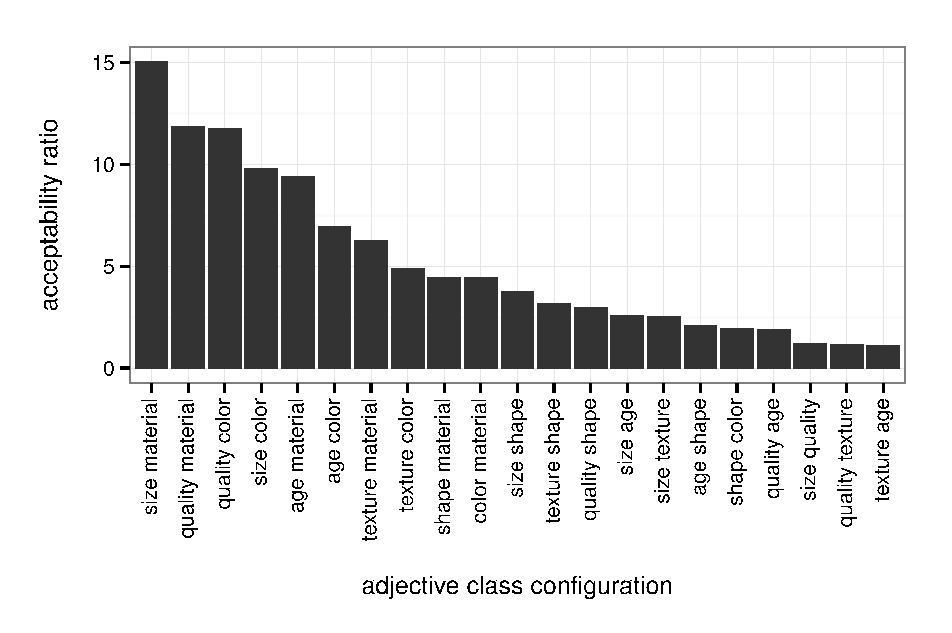
\includegraphics[width=.95\linewidth]{plots/order_ratio.eps}
	\caption{Accpetability ratios for the preferred adjective class orderings.}\label{order-ratio}
\end{figure}

On the basis of these preferred orderings, we may calculate the average distance from noun for each class, plotted in Fig.\ \ref{class-distance}. Comparing Fig.\ \ref{class-distance} with the corpus-based distance scores reported in Fig.\ \ref{distance-from-noun} confirms the reliability of the current paradigm: we replicate near exactly the qualitative order of adjective class distance from noun. 

\begin{figure}[h]
	\centering
	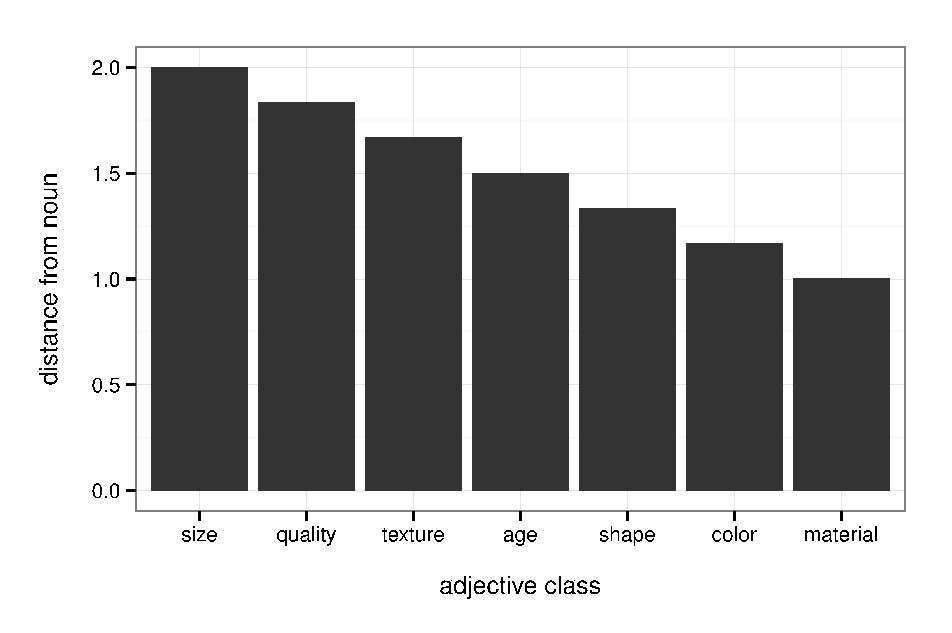
\includegraphics[width=.95\linewidth]{plots/class_distance.eps}
	\caption{Average distance from noun for each adjective class calculated from order preference ratings.}\label{class-distance}
\end{figure}

We may infer the order preferences in \ref{expt-inferred-order-preferences} (cf.\ the preferences inferred from corpus counts in \ref{inferred-order-preferences} above).
\be
size > quality > age > texture > shape > color > material\label{expt-inferred-order-preferences}\ee 
In addition to calculating preference ratios by class configurations, we also calculated preferred orderings for all of the specific adjective pairings. On the basis of how often an adjective from a given class occurred first in an adjective-adjective-noun configuration, we may infer the relative distance from the noun a given class prefers. Fig.\ \ref{class-distance-by-adj} plots these average distance scores, where a value of 2 signals that a class's adjectives always occur first in preferred adjective-adjective-noun orderings, and a value of 1 indicates that a class's adjectives always occur second.

\begin{figure}[h]
	\centering
	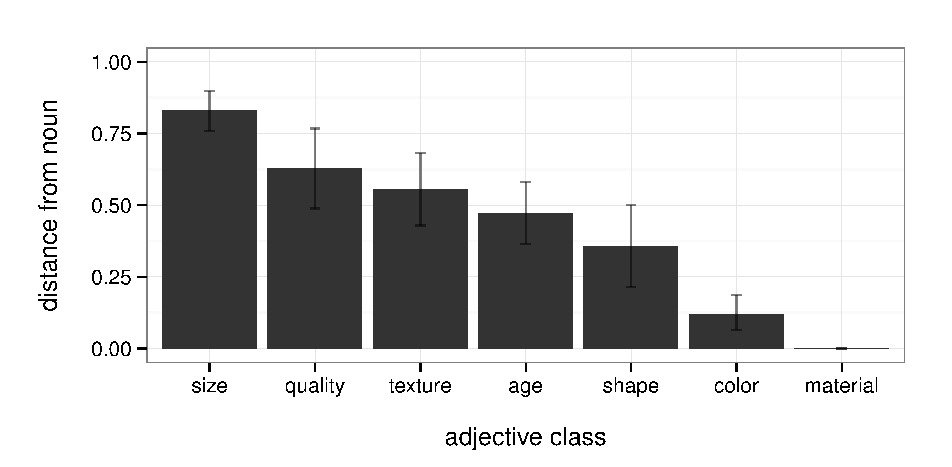
\includegraphics[width=.95\linewidth]{plots/class_distance_by_adj.eps}
	\caption{Average distance from noun for each adjective class by computing how often adjectives from that class occur first in preferred adjective-adjective-noun orderings.}\label{class-distance-by-adj}
\end{figure}

Finally, and most directly related to our hypothesis concerning adjective subjectivity in ordering preferences, we compared acceptability ratings from the current experiment with faultless disagreement scores from Expt.\ 1. To do so, we first calculated a difference score for each class configuration, \textsc{class1}--\textsc{class2}, subtracting the average faultless disagreement score for \textsc{class1} from the average faultless disagreement score for \textsc{class2}. Fig.\ \ref{faultless-order} plots class configuration acceptability ratings against faultless disagreement difference scores.

\begin{figure}[h]
	\centering
	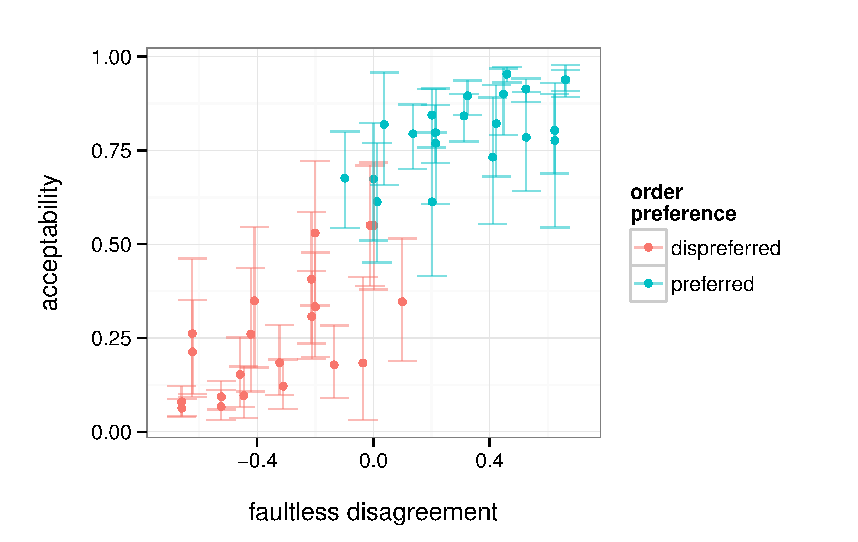
\includegraphics[width=.95\linewidth]{plots/faultless_order_preference.eps}
	\caption{By-class adjective order preferences plotted against difference in faultless disagreement.}\label{faultless-order}
\end{figure}

\section{Discussion}



\begin{materials}
\section{Corpus counts} 

\section{Experiment 1a: Faultless Disagreement}
Something about our methods and how we ran the experiment
\begin{table}[h]
	\caption{Adjectives and nouns used in experimental stimuli.}
	\begin{tabular}{@{\vrule height 10.5pt depth2pt  width0pt}llllll}
	\textbf{adjective}	&	\textbf{class}	&	\textbf{adjective}	&	\textbf{class}	&	\textbf{noun}	&	\textbf{class}	\\ \hline
old	&	age	&	good	&	quality	&	apple	&	food	\\
new	&	age	&	bad	&	quality	&	banana	&	food	\\
rotten	&	age	&	round	&	shape	&	carrot	&	food	\\
fresh	&	age	&	square	&	shape	&	cheese	&	food	\\
red	&	color	&	big	&	size	&	tomato	&	food	\\
yellow	&	color	&	small	&	size	&	chair	&	furniture	\\
green	&	color	&	huge	&	size	&	couch	&	furniture	\\
blue	&	color	&	tiny	&	size	&	fan	&	furniture	\\
purple	&	color	&	short	&	size	&	TV	&	furniture	\\
brown	&	color	&	long	&	size	&	desk	&	furniture	\\
wooden	&	material	&	smooth	&	texture	\\				
plastic	&	material	&	hard	&	texture	\\				
metal	&	material	&	soft	&	texture	\\													
	\end{tabular} \label{stim-table}
\end{table}

\section{Experiment 1b: Subjectivity}

\section{Experiment 2: Ordering preferences}
We recruited 50 participants through Amazon.com's Mechanical Turk crowd-sourcing service. Participants were compensated for their participation.

Participants were asked to indicate which of two descriptions of an object sounded more natural. Each description featured a noun modified by two adjectives, for example ``the red small chair'' or ``the small red chair''. Description pairs contained the same words, with relative adjective order reversed. Descriptions were random combinations of two adjectives and a noun from the list in Table \ref{stim-table} (compiled via the procedure described in Section \ref{corpus}), with the constraint that no description contained adjectives from the same adjective class.
On each trial, participants indicated which description sounded more natural by adjusting a slider whose endpoints were labeled with the competing descriptions; an example trial appears in Fig.\ \ref{order-trial}.

\begin{figure}[h!]
	\centering
	\fbox{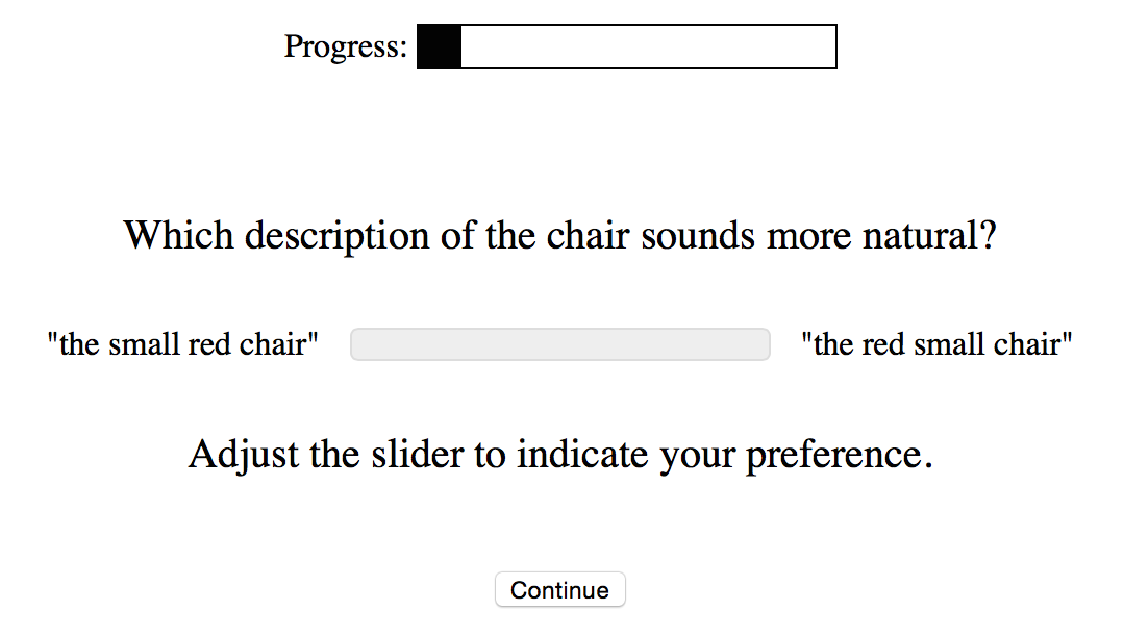
\includegraphics[width=.8\linewidth]{images/order_trial.eps}}
	\caption{Example trial from Expt.\ 1; participants indicated the more natural of two adjective-adjective-noun descriptions on a sliding scale.}\label{order-trial}
\end{figure}

Only native speakers of English with IP addresses located within the United States were included in the analyses; we analyzed data from 45 participants.


\end{materials}

\begin{acknowledgments}
This work was supported in part by Office of Naval Research Grant N000141310788 (to N.D.G.).
\end{acknowledgments}

\begin{thebibliography}{10}
\bibitem{BN}
M.~Belkin and P.~Niyogi, {\em Using manifold structure for partially
  labelled classification}, Advances in NIPS, 15 (2003).

\bibitem{BBG:EmbeddingRiemannianManifoldHeatKernel}
P.~B\'erard, G.~Besson, and S.~Gallot, {\em Embedding {R}iemannian
  manifolds by their heat kernel}, Geom. and Fun. Anal., 4 (1994),
  pp.~374--398.

\bibitem{CLAcha1}
R.R.~Coifman and S.~Lafon, {\em Diffusion maps}, Appl. Comp. Harm. Anal.,
  21 (2006), pp.~5--30.

\bibitem{DiffusionPNAS}
R.R.~Coifman, S.~Lafon, A.~Lee, M.~Maggioni, B.~Nadler, F.~Warner, and
  S.~Zucker, {\em Geometric diffusions as a tool for harmonic analysis and
  structure definition of data. {P}art {I}: Diffusion maps}, Proc. of Nat.
  Acad. Sci.,  (2005), pp.~7426--7431.

\bibitem{Clementi:LowDimensionaFreeEnergyLandscapesProteinFolding}
P.~Das, M.~Moll, H.~Stamati, L.~Kavraki, and C.~Clementi, {\em
  Low-dimensional, free-energy landscapes of protein-folding reactions by
  nonlinear dimensionality reduction}, P.N.A.S., 103 (2006), pp.~9885--9890.

\bibitem{DoGri}
D.~Donoho and C.~Grimes, {\em Hessian eigenmaps: new locally linear
  embedding techniques for high-dimensional data}, Proceedings of the National
  Academy of Sciences, 100 (2003), pp.~5591--5596.

\bibitem{DoGri:WhenDoesIsoMap}
D.~L. Donoho and C.~Grimes, {\em When does isomap recover natural
  parameterization of families of articulated images?}, Tech. Report Tech. Rep.
  2002-27, Department of Statistics, Stanford University, August 2002.

\bibitem{GruterWidman:GreenFunction}
M.~Gr\"uter and K.-O. Widman, {\em The {G}reen function for uniformly
  elliptic equations}, Man. Math., 37 (1982), pp.~303--342.

\bibitem{Simon:NeumannEssentialSpectrum}
R.~Hempel, L.~Seco, and B.~Simon, {\em The essential spectrum of neumann
  laplacians on some bounded singular domains}, 1991.

\bibitem{1}
Kadison, R.\ V.\ and Singer, I.\ M.\ (1959)
Extensions of pure states, {\it Amer.\ J.\ Math.\ \bf
81}, 383-400.

\bibitem{2}
Anderson, J.\ (1981) A conjecture concerning the pure states of
$B(H)$ and a related theorem. in {\it Topics in Modern Operator
Theory}, Birkha\"user, pp.\ 27-43.

\bibitem{3}
Anderson, J.\ (1979) Extreme points in sets of
positive linear maps on $B(H)$. {\it J.\ Funct.\
Anal.\
\bf 31}, 195-217.

\bibitem{4}
Anderson, J.\ (1979) Pathology in the Calkin algebra. {\it J.\
Operator Theory \bf 2}, 159-167.

\bibitem{5}
Johnson, B.\ E.\ and Parrott, S.\ K.\ (1972) Operators commuting
with a von Neumann algebra modulo the set of compact operators.
{\it J.\ Funct.\ Anal.\ \bf 11}, 39-61.

\bibitem{6}
Akemann, C.\ and Weaver, N.\ (2004) Consistency of a
counterexample to Naimark's problem. {\it Proc.\ Nat.\ Acad.\
Sci.\ USA \bf 101}, 7522-7525.

\bibitem{TSL}
J.~Tenenbaum, V.~de~Silva, and J.~Langford, {\em A global geometric
  framework for nonlinear dimensionality reduction}, Science, 290 (2000),
  pp.~2319--2323.

\bibitem{ZhaZha}
Z.~Zhang and H.~Zha, {\em Principal manifolds and nonlinear dimension
  reduction via local tangent space alignement}, Tech. Report CSE-02-019,
  Department of computer science and engineering, Pennsylvania State
  University, 2002.
\end{thebibliography}


\end{article}




\end{document}


